\documentclass{article}
% * <alex.makassiouk@gmail.com> 2018-04-05T14:17:23.414Z:
%
% ^.
\usepackage[utf8]{inputenc}

%% Language and font encodings
\usepackage[english]{babel}
%\usepackage[utf8x]{inputenc}
\usepackage[T1]{fontenc}

%% Sets page size and margins
\usepackage[a4paper,top=3cm,bottom=2cm,left=3cm,right=3cm,marginparwidth=1.75cm]{geometry}

%% Useful packages
\usepackage{float}
\usepackage{graphicx}
\usepackage[colorinlistoftodos]{todonotes}
\usepackage[colorlinks=true, allcolors=blue]{hyperref}

\usepackage[english]{babel}
\usepackage[utf8]{inputenc}
\usepackage{amsmath}
\usepackage{amssymb}
\usepackage{graphicx}
\usepackage[colorinlistoftodos]{todonotes}
\usepackage{scrextend}

\usepackage{hyperref}
\usepackage{tikz-cd}
\usepackage{amsthm}
\usepackage{relsize}
\usepackage{adjustbox}
\usepackage[makeroom]{cancel}
\usepackage[backend=biber,
style=alphabetic,
sorting=ynt]{biblatex}

\usepackage{xifthen}

%\usepackage{titlesec}
%\newcommand{\sectionbreak}{\clearpage}

%\usepackage{showkeys}

\theoremstyle{definition}
\newtheorem{theorem}{Theorem}[section]
\newtheorem{definition}{Definition}[section]
\newtheorem{conjecture}{Conjecture}[section]
\newtheorem{example}{Example}[section]
\newtheorem{exercise}{Exercise}[section]
\newtheorem{problem}{Problem}[section]

\newtheorem{application}{Application}[section]

\newtheorem{construction}{Construction}[section]

%\theoremstyle{plain}
\newtheorem{lemma}[theorem]{Lemma}
\newtheorem{proposition}[theorem]{Proposition}
\newtheorem*{corollary}{Corollary}


\theoremstyle{remark}
\newtheorem*{remark}{Remark}
\newtheorem*{note}{Note}
\title{On Meissel-Mertens constants for polynomials}
\author{Alex Makassiouk, Preben Hast Sørli}


\begin{document}

\maketitle
\author
\begin{center}
Fagerlia VGS, Ålesund
\end{center}

\begin{center}
Submitted to the Norwegian Contest for Young Scientists
\linebreak



\end{center}

\begin{abstract}
\centering
The Meissel-Mertens constant is a famous real number built from the prime numbers. In our project we generalize this and define the Meissel-Mertens constant for any polynomial with integer coefficients. This is motivated by a conjecture of Atle Selberg from 1989. Choosing the polynomial $f(x) = x$ recovers the classical Meissel-Mertens constant as a special case. We investigate our generalized Meissel-Mertens constants, obtaining both computational and theoretical results.

\end{abstract}

\cleardoublepage

\tableofcontents

\clearpage

\section{Introduction}
\subsection{The Meissel-Mertens constant}
Consider the harmonic series:
$$\sum_{k=1}^{\infty}\frac{1}{k}=\frac{1}{1}+\frac{1}{2}+\frac{1}{3}+\frac{1}{4}\cdots$$
From Euler, we know that this sum is divergent, but that
$$\lim_{n\rightarrow\infty} \left(\sum_{k=1}^{n}\frac{1}{k}-\log(n) \right) = \gamma$$
where $\gamma$ is Euler's constant (also called the Euler-Mascheroni constant), which is approximately equal to:
$$0.57721566490153286060651209008240243104215933593992\dots$$
\newline
\newline
If we further consider
$$\sum_{p \text{ prime}}\frac{1}{p}=\frac{1}{2}+\frac{1}{3}+\frac{1}{5}+\frac{1}{7}+\frac{1}{11}\cdots $$
also called the sum of the prime reciprocals, the sum will also diverge. But if we look at the expression  $$\lim_{n\rightarrow \infty } \left (\sum_{p\leq n}\frac{1}{p}\ -\log (\log n) \right )$$ we will se that it converges to a constant in a similar fashion as with the Euler's constant, $\gamma$.
This is what we call the Meissel-Mertens constant and it is named after Ernst Meissel and Franz Mertens. An  approximation to the constant is: $$M \approx 0.2614972128476427837554268386\dots$$
The fascinating thing about the Meissel-Mertens constant is that it behaves in the exact same way as Euler's constant, but instead of a straight forward $\frac{1}{k}$ sum we use the prime reciprocals and the double log instead of a single log.


\subsection{Generalising the Meissel-Mertens constant to polynomials}

The current project is based on a suggestion from our math teacher:
\vskip12pt
\begin{addmargin}{1cm}
\it One of the most fundamental problems of mathematics is the question "How many primes are there". Possible answers to this question range in sophistication from the very easy fact that there are infinitely many primes, to the exceptionally difficult (and still unproven!) Riemann hypothesis, which gives a very precise answer to how many primes there are up to any given bound. An intermediate statement (much stronger than the first, and much weaker than the second) is the existence of a certain limit called the Meissel-Mertens constant. This statement is particularly interesting for two reasons. First, it can be proven using only real analysis (i.e. no complex-analytic functions). Secondly, mathematicians expect that the Riemann hypothesis holds in much more general examples than the classical setting of ordinary prime number theory, and in these other settings, it seems like no-one has investigated the existence and properties of Meissel-Mertens constants (although their existence probably follows from things that are known to number theory experts). In these more general settings, there is some motivation coming from a famous conjecture of Atle Selberg. Maybe it is possible to learn about the Meissel-Mertens constant, and to investigate some new forms of "generalized Meissel-Mertens constants" using the tools of real analysis that you already know? %This would be closely related to a famous conjecture of Atle Selberg on "orthonormality of functions in the Selberg class", but you don't really need to understand what this conjecture says except in some special cases.
\end{addmargin}
\vskip12pt

In this project, we define a generalized Meissel-Mertens constant for any polynomial with integer coefficients as we will now describe.
\begin{definition}
For any prime $p$ we set $\mathbb{Z}/p$ to denote the ring of integers modulo $p$.
\end{definition}

\begin{definition}\label{defF}
Let F be a polynomial with integer coefficients. Then we define
$a_p(F)$ as the number of roots to the polynomial $F$ in $\mathbb{Z}/p$.
\end{definition}

\begin{definition}\label{defS(F,n)}
With F and $a_p(F)$ as in Definition \ref{defF}, and for any positive integer $n$ we define
$$S(F,n) = \frac{\sum_{p\leq n}\frac{a_p^2}{p}}{\log(\log(n))} $$
where the sum is taken over all primes up to $n$.
\end{definition}

\begin{conjecture}
With $S(F,n)$ as in \ref{defS(F,n)}, the following limit exists and is a positive integer:
$$\lim_{n\rightarrow \infty} S(F,n) $$
\end{conjecture}

\begin{definition}
When the preceding limit exists, we denote it by $S(F)$.
\end{definition}

\begin{definition}
Asssuming that $S(F)$ exists, we define:
$$M(F,n) = \sum_{p\leq n}\frac{a_p^2}{p} - S(F)\cdot \log(\log(n)) $$
\end{definition}

\begin{conjecture}
For any polynomial $F$ with integer coefficients, the limit $$\lim_{n \rightarrow \infty } M(F,n)$$
exists.
\end{conjecture}

\begin{definition}
Assuming the preceding conjecture, we define
$$M(F)=\lim_{n \rightarrow \infty} M(F,n)$$
\end{definition}

%We find that we need to use the Selberg inner product $S$ when we try to find the Meissel-Mertens constant for a given polynomial. Without it M will unfortunately not converge. We need to find a whole number which we put in front of $log(log(n))$ and that is the Selberg inner product, which acts like a scalar product formula for polynomials instead of vectors, where we use the Riemann zeta function as one of the polynomials and vary the second. \todo[inline]{The Selberg Inner product has to be much better defined than this. }
The definition of $S(F)$ is inspired by a conjecture of the Norwegian mathematician Atle Selberg from 1989, which you can read more about in Murty [\ref{refMurty}]. This conjecture concerns sequences of numbers $a_p$ similar to the ones we deal with in this project. However, the definition of $M(F)$ given here is not found anywhere in the literature as far as we know.

\subsection{Problem formulation}
\begin{enumerate}

\item Prove that the limits $S(F)$ and $M(F)$ exists for as many polynomials as possible.

\item How do we compute $S(F)$ and $M(F)$ numerically?

\item Lastly, how can we use our numerical results, and do we see any patterns in them which could be investigated in future research?

\end{enumerate}

\subsection{Method}


We divide our method part in two. We have theoretical and computational methods.
The theoretical methods are as follows:
\begin{enumerate}
\item Reading relevant references
\item Discussions with experts (Henri Cohen and others)
\item Finding and writing down proofs
\end{enumerate}
The computational methods are:
\begin{enumerate}
\item Numerical experiments in SageMath:
We started our project using SageMath, available on the online platform CoCalc. Here we laid down the first code for both $S(F)$ and the Meissel-Mertens constant. SageMath (System for Algebra and Geometry Experimentation) is a computer algebra system covering many aspects of mathematics, including algebra, combinatorics, graph theory, numerical analysis and number theory. The originator and leader of the SageMath is William Stein
\item Numerical experiments in PARI/GP:
After a while we found that CoCalc became too slow for computing our problems for very high values. We would then optimize our code to make it faster, but we also found that PARI/GP would be a more efficient programmable calculator.
\newline
PARI/GP is a computer algebra system for computations in number theory, developed by Karim Belabas and Henri Cohen at Université Bordeaux, and it is written in C. PARI is the C library, while GP is the easy-to-use interactive command line interface giving access to the PARI library, containing many of the number theoretical functions we use.
\end{enumerate}
We also did an excursion to a PARI/GP-workshop in the Blaise-Pascal university. Here we met Henri Cohen and other experts who introduced us to PARI and gave us some theoretical clues and relevant references.

\subsection{Results}
\begin{itemize}
\item We present a way to calculate the original Meissel-Mertens constant with extremely high precision using very little computing power. The main underlying theoretical result is the following relation:
$$M = \gamma + \sum_{m\geq 2}\frac{\mu(m)}{m} \cdot \log(\zeta(m))$$
where $M$ is the original Meissel-Mertens constant, $\gamma$ is Euler-Mascheroni constant, $\mu$ is the Möbius function and $\zeta$ is the Riemann zeta function.
\item We prove that for any linear polynomial $F$ we have $S(F)=1$ and that if $F$ is furthermore monic, then $M(F)$ equals the classical Meissel-Mertens constant.
\item We present a formula for counting roots in $\mathbb{Z}/p$ for any irreducible monic polynomial of degree two, and by utilizing this formula we prove that for these specific polynomials we have $S(F)=2$.
\item We prove that for any monic quadratic reducible polynomial $F$, we have:
\begin{enumerate}
\item  $S(F)=1$ if the discriminant is $0$.
\item $S(F)=4$ if the discriminant is not $0$.
\end{enumerate}
\item We prove that the limit $M(F)$ exists for any monic quadratic polynomial.
\item Based on our theoretical results we write simple programs for numerical approximation of $S(F,n)$ and $M(F,n)$.
\end{itemize}


\subsection{Acknowledgements}
We thank our teacher Andreas Holmström, the team behind PARI/GP (Bill Allombert, Henri Cohen, Karim Belabas, Nicolas Billerey), and we would extend our gratitude to our fellow students Torstein Vik, Magnus Hellebust Haaland, and Olav Hellebust Haaland. Thank you to SageMath and PARI/GP for excellent software, and Overleaf for LaTeX editing. Last but not least we want to thank our school Fagerlia videregående skole, its principal Yngve Omenås and Head of natural sciences, Ivar Karsten Lerstad. We especially want to thank the school for financing our trip to the PARI/GP-workshop where we learned to use our computational tool which has been critical to this project.
\newpage
\section{Background knowledge}
\subsection{Notation}
\begin{itemize}
\item $\log:$ The natural logarithm with Euler's number $e$ as base.
\item $a_p:$ Number of solutions to a polynomial modulo $p$
\item $\mathbb{Z}/p$: The ring of integers modulo $p$.
\item $x:$ Denotes a real variable
\item $X:$ Denotes a formal variable used in polynomials
\item $\mathbb{Z}$: The set of integers.
\item $\mathbb{P}:$ The set of all primes
\item $p$: Any prime.
\item $\gamma:$ The Euler-Mascheroni constant (also called Euler's constant)
\item $\zeta(x):$ The Riemann zeta function
\item $G(x):$ The prime zeta function, an analogue of the Riemann zeta function
\item $D:$ Limit as $x$ goes to $1$ of $\log(\zeta(x))-G(x)$ (more details later)
\item $\chi$: denotes a Dirichlet character.
\item $\mathcal{O}$: This is called big-O notation and "describes the limiting behavior of a function when the argument tends towards a particular value or infinity." \footnote{From Wikipedia article on Big O notation} Wikipedia states a formal definition:
\begin{definition}
Let $f$ and $g$ be two functions defined on some subset of the real numbers. One writes

$$f(x)=\mathcal{O}(g(x))\text{ as }x\to\infty$$

if and only if there exists a positive real number $C$, called "the implicit constant", and a real number $x_0$ such that

$$|f(x)| \leq  C |g(x)|\text{ for all }x \geq x_0$$

Similarly, we write
$$f(x)=\mathcal{O}(g(x)) \text{ as }x \to a$$
if and only if there exists a positive real number $C$, called "the implicit constant", and a real number $x_0$ such that

$$|f(x)| \leq  C |g(x)|\text{ for all }x \text{ such that } \vert x-a\vert < x_0$$
\end{definition}
\item $\mu:$ The Möbius function
\item When we write,
$$\sum_pf(p)$$
the notation will always mean that we sum the expression $f(p)$ over all prime numbers.
\item $\equiv$ : The congruence relation from modular arithmetic. $A \equiv B $ (mod p) if $\frac{A}{p} = k + \frac{B}{p}$ for some integer k.
\item $n|m$: This reads "$n$ divides $m$", and means $n$ is a divisor of $m$.
\end{itemize}

\subsection{Polynomials}
\begin{definition}
\textbf{Reducible polynomials}
Polynomials that can be factored using only integers, such as $X^2-1$, will simply be referred to as reducible polynomials.
\end{definition}
\begin{definition}
\textbf{Irreducible polynomials.}
Polynomials that cannot be factored using integers will be referred to as irreducible polynomials.
\end{definition}
\begin{definition}
\textbf{Monic polynomials}
A polynomial is called monic, if the coefficient of the term of highest degree is $1$.
\end{definition}

\subsection{Number-theoretic functions}
\subsubsection{Legendre symbols}
\begin{definition}\label {defLegendre}
We write the Legendre symbol as $(\frac{a}{p})$ and it is defined, for all integers $a$ and odd primes $p$, as the following:
$$\left(\frac{a}{p}\right) = \begin{cases}
0  & \text{if } a \equiv 0\pmod{p} \\
1 & \text{if } a \not\equiv 0\pmod{p} \text{ and for some integer } x\colon\;a\equiv x^2\pmod{p},\\
-1 & \text{if } a \not\equiv 0\pmod{p} \text{ and there is no such } x.
\end{cases}$$
\end{definition}


\subsubsection{Kronecker symbols}
\begin{definition}\label{defKronecker}
The Kronecker symbol is a generalisation of the Legendre symbols, which we write as $(\frac{a}{n})$ and for odd primes in $n$ the Kronecker symbol is defined exactly the same as the Legendre symbol. In addition the Kronecker symbol is also defined for the case $p=2$.
\newline
The Kronecker symbol $(\frac{a}{2})$ is defined as the following:
$$\left(\frac{a}{2}\right) = \begin{cases}
& 0 \text{ if } a \text{ is even } \\
& 1 \text{ if } a \equiv \pm1 \pmod{8} \\
& -1 \text{ if } a \equiv \pm3 \pmod{8} \\
\end{cases}$$
\end{definition}
The decisive reason for using the Kronecker symbol instead of Legendre, is the easy implementation of the Kronecker symbol in PARI, and especially what we find in Theorem \ref{kronecker}

\subsubsection{The Möbius function}
\begin{definition}
For any positive integer $n$ Wikipedia \footnote{See the Wikipedia article on the Möbius function in the bibliography} defines the Möbius function as following:
\begin{itemize}
\item $\mu(n)= 1$ if $n$ is a square-free positive integer with an even number of prime factors.
\item $\mu(n)= -1$ if $n$ is a square-free positive integer with an odd number of prime factors.
\item $\mu(n)= 0$ if $n$ has a squared prime factor.
\end{itemize}
\end{definition}

\subsubsection{Dirichlet characters}
\begin{definition}
A Dirichlet character is a function $\chi:\mathbb{Z}\rightarrow \mathbb{C}$
 such that:\footnote{From the Wikipedia article on Dirichlet characters.}

 \begin{enumerate}
 \item There exists a positive integer $k$ such that $\chi(n) = \chi(n + k)$ for all $n$.
 \item If $gcd(n,k) > 1$ then $\chi(n) = 0$; if $gcd(n,k) = 1$ then $\chi(n) \neq 0$.
 \item $\chi(m\cdot n) = \chi (m) \cdot \chi (n)$ for all integers $m$ and $n$.
\item $\chi(1)=1$
\end{enumerate}
\end{definition}

\subsection{Zeta functions}

In this document we only use a real variable $x$ although our definitions and results also sometimes hold for complex variables.
\begin{definition} \label{defRiemannZeta}
We define the Riemann zeta function
$$\zeta(x)=\sum_{n=1}^{\infty}\frac{1}{n^x}$$
\end{definition}
\begin{proposition}
$\zeta(x)$ is absolutely convergent for $x>1$.
\end{proposition}
\begin{proposition}
For any $x > 1$, we have the Euler product formula: \footnote{See the Wikipedia article on the Riemann zeta function}
$$\sum_{n=1}^{\infty}\frac{1}{n^x}=\prod_p\frac{1}{1-p^{-x}}$$
\end{proposition}
\begin{proof}
This is well known. See for example Wikipedia \footnote{\url{https://en.wikipedia.org/wiki/Proof_of_the_Euler_product_formula_for_the_Riemann_zeta_function}} which also show the previous proposition.
\end{proof}
\begin{definition} \label{defPrime_Zeta}
We define the prime zeta function\footnote{See the Wolfram article on the Prime zeta function}, an analogue of the Riemann zeta function, as:
$$G(x)=\sum_p \frac{1}{p^{x}}$$
\end{definition}



\begin{definition}
A Dirichlet L-function is a function of the form:
$$L(x,\chi) = \sum_{n=1}^{\infty}\frac{\chi(n)}{n^x}$$
associated to the Dirichlet character $\chi$
\end{definition}

\subsection{The Euler-Mascheroni constant}
\begin{definition}
The Euler-Mascheroni constant is defined by
$$\gamma = \lim_{n \rightarrow \infty} \left( 1 + \frac{1}{2} + \cdots + \frac{1}{n} - \log n \right)$$
\end{definition}
In our computations we use the built in Euler-Mascheroni constant in PARI, but the following proposition could also be used to compute $\gamma$ with high precision.
\begin{proposition}
$$\gamma = \frac{3}{2}-\log2-\sum_{m=2}^{\infty}(-1)^m\frac{m-1}{m}(\zeta(m)-1) $$
\end{proposition}
\begin{proof}
See Flajolet and Vardi[\ref{refFlajolet}].
\end{proof}
\begin{proposition}\label{Tenenbaum 0.5}
For $n \geq 1$, we have
$$\sum_{m\leq n}\frac{1}{m}= \log(n) + \gamma + \frac{1}{2n}-\frac{1}{12n^2}+\frac{\theta}{60n^4}$$
where $\theta=\theta_n \in [0,1]$.
\end{proposition}
\begin{proof}
See page 6 in Tenenbaum's Introduction to Analytic and Probabilistic Number Theory. The key idea of the proof is to use the Euler-Maclaurin summation formula.
\end{proof}

\begin{proposition}\label{gammaSondow}
%$$\zeta(x)-\frac{1}{x-1}-\gamma=\mathcal{O}(x-1)$$
%as $x$ approaches $1$ from above
We have the relation:
$$\gamma = \lim_{x \rightarrow 1^+} \left( \zeta(x) - \frac{1}{x-1} \right)$$
\end{proposition}

\begin{proof}
Following Jonathan Sondow [\ref{sondowRef}], we will prove that Euler's constant, $\gamma $ originally defined by
\begin{equation} \label{gammaOrig}
\gamma = \lim_{n \rightarrow \infty} \left( 1 + \frac{1}{2} + \cdots + \frac{1}{n} - \log n \right)
\end{equation}
can be written as
\begin{equation} \label{gammaNew}
 \gamma = \lim_{x \rightarrow 1^+} \left( \zeta(x) - \frac{1}{x-1} \right)
 \end{equation}
we know from definition \ref{defRiemannZeta} that
$$ \zeta(x) = \sum_{n=1}^{\infty} \frac{1}{n^x}$$
Further, we can rewrite
$$\frac{1}{x-1} = \sum_{n=1}^{\infty} \frac{1}{x^n}$$ for $x>1$. That gives us

$$ \gamma = \lim_{x \rightarrow 1^+} \left( \zeta(x) - \frac{1}{x-1} \right) = \lim_{x \rightarrow 1^+} \left( \sum_{n=1}^{\infty} \frac{1}{n^x} - \sum_{n=1}^{\infty} \frac{1}{x^n}\right)$$
$$ = \lim_{x \rightarrow 1^+}\left( \sum_{n=1}^{\infty} \left( \frac{1}{n^x} - \frac{1}{x^n} \right)\right)$$

Now we look back to the original definition of $\gamma$. We can rewrite it to $$ \gamma = \lim_{n\rightarrow \infty} \left( \sum_{k=1}^{n} \frac{1}{k} - \log(n+1) \right)$$

because
$$ \lim_{n\rightarrow \infty} \left(\log(n) - \log(n+1)\right) = \lim_{n\rightarrow \infty} \log\left( \frac{n}{n+1} \right) = 0$$

Now we go back to what we started with and write
$$ \frac{1}{x-1} = \int_{1}^{\infty} \frac{dt}{t^x} = \sum_{n=1}^{\infty}\int_{n}^{n+1} \frac{dt}{t^x} $$ i.e. a sum of small integrals. We can write $\log(n+1)$ in a similar way
$$ \log(n+1) = \int_{1}^{n+1}\frac{dt}{t} = \sum_{k=1}^{n} \int_{k}^{k+1} \frac{dt}{t}$$

It follows that the limits in equations (\ref{gammaOrig}) and (\ref{gammaNew}) can be written as
\begin{equation}
\gamma = \sum_{n=1}^{\infty}\left(\frac{1}{n}-\int_{n}^{n+1}\frac{dt}{t}\right)
\end{equation}
and
\begin{equation}
\gamma = \lim_{x \rightarrow 1^+} \sum_{n=1}^{\infty}\left(\frac{1}{n^x}-\int_{n}^{n+1}\frac{dt}{t^x}\right)
\end{equation}

respectively.

\end{proof}
\newpage

\section{Linear polynomials}

In this section we present some of the work we have done with linear polynomials. This involves much of the fundamental work which will be used later in section 4 as well for quadratic polynomials. We will refer to the classical Meissel-Mertens constant a couple of times, and that is the constant we presented in Section 1.1.
\newline
As the structure of this section we will first use a naive algorithm to compute approximations to the classical Meissel-Mertens constant. After this we will investigate theory which will help us compute the classical Meissel-Mertens constant much faster. After the theoretical part we dedicate a subsection to present the results from our computations.
\subsection{Theoretical results for linear polynomials}
\begin{theorem}
For $x\geq 2$, we have
$$\sum_{p\leq x }\frac{\log p}{p}-\log (x)= \mathcal{O}(1)$$
The term $\mathcal{O}(1)$ lies in the open interval
$$]-1-\log 4, \log 4 [ $$
\end{theorem}
\begin{proof}
See Theorem 7 in Tenenbaum, page 14 [\ref{refTenenbaum}]
\end{proof}

\begin{theorem} \label{Thm9Tenenbaum}
There exists a constant $M$ such that, for $x\geq 2$, one has that
$$\sum_{p\leq x}\frac{1}{p}-\log(\log(x))-M=\mathcal{O}\left(\frac{1}{\log x}\right).$$
When $x$ goes to infinity.

We can choose the implicit constant $C$ as $2+2\log 4$ for  the right side of the identity.
\end{theorem}
\begin{proof}
See Theorem 9 in Tenenbaum, page 16 [\ref{refTenenbaum}]
\end{proof}

\begin{lemma}\label{S is 1}
We have the relation
$$\lim_{n \rightarrow \infty }\left(\frac{\sum_{p \leq n}\frac{1}{p}}{\log(\log(n))}\right)=1$$
\end{lemma}
\begin{proof}
We see from Theorem \ref{Thm9Tenenbaum} that the sum
$$\sum_{p \leq n}\frac{1}{p}$$
can be written as
$$\log(\log(n))+M+\mathcal{O}\left(\frac{1}{\log n}\right)$$
Now we want to prove
$$\lim_{n \rightarrow \infty }\left(\frac{\log(\log(n))+M+\mathcal{O}\left(\frac{1}{\log n}\right)}{\log(\log(n))}\right)=1$$
We can rewrite the left-hand side as
$$\lim_{n \rightarrow \infty}\left(\frac{\log(\log(n))}{\log(\log(n))}\right)+\lim_{n \rightarrow \infty}\left(\frac{M}{\log(\log(n))}\right)+\lim_{n \rightarrow \infty}\left(\frac{\mathcal{O}(\frac{1}{\log(n)})}{\log(\log(n))}\right)$$
which is clearly equal to
$$1+0+0$$
\end{proof}

\begin{corollary}
For $F(X) = X+c$ the limit S(F) exists and is 1.
\end{corollary}
\begin{proof}
For these polynomials $a_p=1 \quad \forall \quad p$. From Lemma \ref{S is 1} we see that $S(F)=1$.
\end{proof}
\begin{corollary}
For $F(x)=aX+c$ the limit $S(F)$ exists and is $1$.
\end{corollary}
\begin{proof}
When $p$ does not divide $a$, there is one solution to the congruence
$$F(X) \equiv 0 \pmod{p}$$
because in that case $a$ is invertible in $\mathbb{Z}/p$.
When $p$ divides $a$, this is not necessarily the case, but by argument similar to the one given later in the proof of Theorem \ref{preben1}, this finite set of primes does not affect $S(F)$.
\end{proof}

\begin{proposition}
Let $F(X) = X + c$, then $M(F)$ equals the classical Meissel-Mertens constant
\end{proposition}
\begin{proof}
The number of solutions to $F(X)$ in $\mathbb{Z}/p$ is $1$ for all $p$.
\end{proof}

\subsection{Computational results with the naive algorithm}

Our naive method for calculating M is simply to sum the first terms such that $p\leq x$ for some fixed x.
$$\sum_{p\leq x}\frac{1}{p}-\log\left(\log(x)\right)$$
for some number x.
We will now present our first computational results. This is of course the simplest case with the simplest programming where we compute the expression above in the most naive way possible:
\begin{figure}[H]
\centering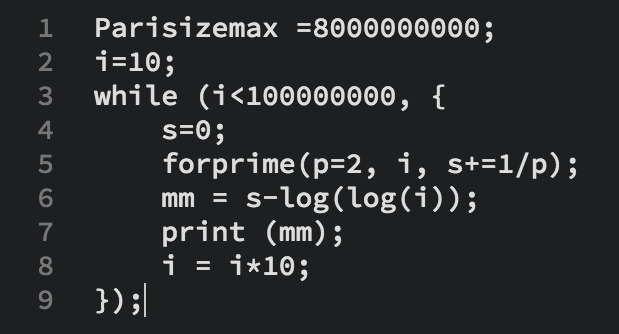
\includegraphics[width = 0.7 \textwidth]{classicalMCode.png}
\caption{\label{fig: ClassicalM} Naive code for classical Meissel-Mertens constant}
\end{figure}
We use a loop where we loop through n-values of the form $n^k$ to see how the convergence behaves for the following expression:
$$\sum_{p\leq n}\frac{1}{p}-\log\left(\log(n)\right)$$
The results the code above will give:

\begin{table}[H]
\centering
\label{ClassicalMTable}
\begin{tabular}{|l|l|}
\hline
$n$                    & $M(F,n)$                                                             \\ \hline
$10$                   & $0.34215803094252039067297742833293709497 $
			\\ \hline
$10^2$ & $0.27563757524096983065117065657078325230$                     \\ \hline
$10^3$ & $0.26543539325902205039001850386165690642$                      \\ \hline
$10^4$ & $0.26273314086571421746193404412499271298$                      \\ \hline
$10^5$ & $0.26180182136520797363858367362229105189$                      \\ \hline
$10^6$ & $0.26153618509166191173232089277122871732$                      \\ \hline
\end{tabular}
\caption{Classical Meissel-Mertens constant for different n-values }
\end{table}

\subsection{Theory for faster computation}
This subsection contains a well-known but ingenious rewrite for the classical Meissel-Mertens constant. Through various steps, we show that the Meissel Mertens constant can be expressed in such a way that our computations converge must faster. Suddenly we are able to compute with several hundred correct decimal points in seconds -- as opposed to letting the computer run for several minutes to get three correct decimal points.


The aim of this subsection is to prove the following theorem. This argument is partly due to an explanation from Henri Cohen and partly due to Tenenbaum's book, \textit{Introduction to Analytic and Probabilistic Number Theory}.
\begin{theorem} \label{fasterMTheorem}
We have the relation:
$$M=\gamma+\sum_{m\geq 2} \frac{\mu(m)}{m}\cdot \log(\zeta(m))$$
\end{theorem}

\begin{lemma}\label{Sum leq zeta}
The sum
$$\left(\sum_p\left(\frac{(p^{-x})^2}{2}+\frac{(p^{-x})^3}{3}\cdots \right)\right)$$
is absolutely convergent for $x\geq 1$.
\end{lemma}
\begin{proof}
We write $t$ for $p^x$ and get:
\begin{equation}
\begin{split}
& \sum_p\left(\frac{1}{2t^2}+\frac{1}{3t^3}+\frac{1}{4t^4}\cdots \right) \\
< \quad & \sum_p \left(\frac{1}{t^2}+\frac{1}{t^3}+\frac{1}{t^4} \cdots \right) \\
= \quad & \sum_p \left(\frac{1}{t^2}\cdot (1+\frac{1}{t}+\frac{1}{t^2}\cdots) \right)  \\
= \quad & \sum_p \left(\frac{1}{t^2}\cdot \frac{1}{1-\frac{1}{t}} \right) \\
= \quad & \sum_p \left(\frac{1}{t(t-1)} \right) \\
< \quad & \sum_p \left(\frac{1}{(t-1)^2} \right) \\
< \quad & \sum_p \left(\frac{1}{(p-1)^2} \right) \\
< \quad & \sum_{k=1}^{\infty}\frac{1}{k^2} \\
= \quad & \zeta(2)
\end{split}
\end{equation}
We see that all terms in our sum are less than or equal to the terms in the sum $\sum_n\frac{1}{n^2}$, which we know to be $\zeta(2)$, which is $\frac{\pi^2}{6}$. From this we can conclude that the sum
$$\sum_p\left(\frac{(p^{-x})^2}{2}+\frac{(p^{-x})^3}{3}\cdots \right)$$
converges, and our proof is complete.
\end{proof}

\begin{definition} \label{def1.1}
$$D=\sum_p\left(\frac{1}{2p^2}+\frac{1}{3p^3}+\frac{1}{4p^4}\cdots \right)$$
\end{definition}

\begin{lemma}\label{logzeta-G}
The limit
$$\lim_{x\rightarrow 1^+}\left(\log(\zeta(x))-\sum_p\frac{1}{p^x} \right)$$
exists and is equal to $D$.
\end{lemma}
\begin{proof}
From Euler's product formula for the Riemann zeta function we can write
\begin{equation}
\begin{split}
& \lim_{x\rightarrow 1^+}\left(\log(\zeta(x))-\sum_p\frac{1}{p^x} \right) \\
 = & \lim_{x\rightarrow 1^+} \left( \log \prod_p \frac{1}{1-p^{-x}}-\sum_p\frac{1}{p^x} \right) \\
 = & \lim_{x\rightarrow 1^+} \left(-\sum_p \log(1-p^{-x})- \sum_p\frac{1}{p^x} \right)\\
 = & \lim_{x\rightarrow 1^+} \left(-\sum_p\left(\log(1-p^{-x})+\frac{1}{p^x} \right)\right) \\
 = & \lim_{x\rightarrow 1^+} \left(-\sum_p\left(-p^{-x}-\frac{(p^{-x})^2}{2}-\frac{(p^{-x})^3}{3}\cdots+\frac{1}{p^x} \right)\right) \\
 = & \lim_{x\rightarrow 1^+} \left(-\sum_p\left(-\frac{(p^{-x})^2}{2}-\frac{(p^{-x})^3}{3}\cdots \right)\right)
\end{split}
\end{equation}
In the second step we use the product rule for logarithms to rewrite the logarithm of the Euler product and get another sum. We now have two sums over $p$ and in the third step we  write this as one sum with two terms. In the next step the Taylor series for the natural logarithm lets us write the sum without the natural logarithm, and we use this in the final step to see that the term $\frac{1}{p^x}$ cancel out. Continuing, we see that
\begin{equation}
\begin{split}
& \lim_{x\rightarrow 1^+} \left(\sum_p\left(\frac{(p^{-x})^2}{2}+\frac{(p^{-x})^3}{3}\cdots \right)\right) \\
= &  \sum_p \lim_{x\rightarrow 1^+}\left(\frac{(p^{-x})^2}{2}+\frac{(p^{-x})^3}{3}\cdots \right) \\
= & \sum_p \left(\frac{p^{-2}}{2}+\frac{p^{-3}}{3}\cdots \right)
\end{split}
\end{equation}



From lemma \ref{Sum leq zeta}, we know that this is equal to $D$.
\end{proof}
Our next goal is to prove Proposition \ref{D-formula} using three lemmas as intermediate step.

\begin{lemma}\label{moebius lik 0}
\begin{equation}
\sum_{m\vert K}\mu(m) = 0 \quad \forall \quad K>1
\end{equation}
\end{lemma}
\begin{proof}
%We can write
%$$K=p_{1}^{e_1}\cdotp_{2}^{e_2}\cdots p_{r}^{e_r}$$
%where $r$ is the number of prime factors of $K$.
%If $r=1$, we get $K=p^e$ and
%$$\sum_{m \vert K}\mu(m)=\mu(1)+\mu(p)+\mu(p^2)\cdots + \mu(p^e) = 1+(-1) = 0$$
For $K=p^r$, a prime power, the sum is equal to $\mu(1)+\mu(p)=1-1=0$. One can show that
$$\sum_{m \vert K}\mu(m)$$
is multiplicative as a function of $K$. Hence, the lemma follows for all $K > 1$.
\end{proof}

\begin{lemma} \label{G to moebius}
Recall the prime zeta function $G(x)$ defined in definition \ref{defPrime_Zeta}. If $x>1$
$$G(x)=\sum_{m\geq 1}\frac{\mu(m)}{m}\cdot \log(\zeta(mx))$$
\end{lemma}
\begin{proof}
First we see that %by the Euler product formula
\begin{equation} \label{eq3}
\begin{split}
\log(\zeta(mx)) & = \log \prod_p \frac{1}{1-p^{-mx}} \\
 & = -\sum_p \log(1-p^{-mx}) \\
 & = -\sum_p(-p^{-mx}-\frac{p^{-2mx}}{2}-\frac{p^{-3mx}}{3}\cdots)\\
 & = \sum_p(p^{-mx}+\frac{p^{-2mx}}{2}+\frac{p^{-3mx}}{3}\cdots) \\
 & = \sum_p\sum_{k\geq 1}\frac{p^{-kmx}}{k} \\
 & = \sum_{k\geq 1} \sum_p \frac{1}{k\cdot p^{kmx}} \\
 & = \sum_{k\geq 1} \frac{1}{k}\cdot \sum_p \frac{1}{ p^{kmx}} \\
 & = \sum_{k\geq 1} \frac{1}{k}\cdot G(kmx)
\end{split}
\end{equation}
Here the first step comes from the Euler product expression for the Riemann zeta-function. The remainding steps are straight-forward rewrites.
\newline
Now we compute

\begin{equation} \label{eq4}
\begin{split}
\sum_{m\geq 1}\frac{\mu(m)}{m}\cdot \log(\zeta(mx)) & = \sum_{m\geq 1}\frac{\mu(m)}{m}\cdot  \sum_{k\geq 1} \frac{1}{k}\cdot G(kmx) \\
& = \sum_{m\geq 1}  \sum_{k\geq 1}\frac{\mu(m)\cdot G(kmx)}{km} \\
& = \sum_{K\geq 1}\frac{G(Kx)}{K}\sum_{m\vert K}\mu(m) \\
& = G(x)
\end{split}
\end{equation}

In the third step we use the substitution $K=km$. We also see in the fourth step that, from Lemma \ref{moebius lik 0} every term in our sum will be zero except for $K=1$, and therefore we have proven the Lemma.
\end{proof}

\begin{lemma} \label{prop G - logZeta}
If $x > 1$, we have the relation
$$G(x)-\log(\zeta(x)) = \sum_{m\geq 2} \frac{\mu(m)}{m}\cdot \log(\zeta(mx))$$
\end{lemma}

\begin{proof}
We know from lemma \ref{G to moebius} that
$$G(x)=\sum_{m\geq 1}\frac{\mu(m)}{m}\cdot \log(\zeta(mx))$$
We take out the term corresponding to $m=1$
$$G(x)=\sum_{m\geq 2}\frac{\mu(m)}{m}\cdot \log(\zeta(mx))+\log(\zeta(x))\cdot \frac{\mu(1)}{1}$$
Because $\mu(1)=1$ the rest is trivial; we can just move the second term to the left side.
\end{proof}

\begin{proposition}\label{D-formula}
We have the identity:
$$-D=\sum_{m\geq 2} \frac{\mu(m)}{m}\cdot \log(\zeta(m))$$
\end{proposition}


\begin{proof}
From Lemma \ref{logzeta-G} we get:
$$-D=\lim_{x\rightarrow 1^+}\left(\sum_p\frac{1}{p^x}-\log(\zeta(x))  \right)$$
From lemma \ref{prop G - logZeta} we get
$$\lim_{x\rightarrow 1^+}\left(\sum_p\frac{1}{p^x}-\log(\zeta(x))  \right)=\lim_{x \rightarrow 1^+} \left(\sum_{m\geq 2}\frac{\mu(m)}{m}\cdot \log \zeta(mx) \right)$$
When we let $x$ go to $1$, we see that our identity holds.
\end{proof}
Remark: Strictly speaking we have not justified interchanging the limit and the sum in the previous proof, but this can be done.
\newline
In order to prove Theorem \ref{fasterMTheorem}, we still need to prove $M=\gamma - D$. Here we follow Tenenbaum (page 18). We introduce three auxiliary functions, $H$, $P$ and $f$.
\begin{definition}\label{defH(t)}
For any positive real number $t$, we define.
$$H(t)=\sum_{1\leq n \leq t}\frac{1}{n}$$
\end{definition}
\begin{lemma}
For $t\geq1$, we have:
$$H(t)=\log(t)+\gamma+\mathcal{O}(\frac{1}{t})$$
as $t$ goes to infinity.
\end{lemma}
\begin{proof}
This follows from Proposition \ref{Tenenbaum 0.5}.
\end{proof}
\begin{definition}\label{defP(u)}
For any positive real number $u$, we define:
$$P(u)=\sum_{p\leq u}\frac{1}{p}$$
\end{definition}
\begin{lemma} \label{alex1}
If $$g(x) \leq \log \left(\frac{1}{x} + C\right)$$ then $$g(x) \leq \log \left(\frac{1}{x}\right) + Cx$$
\end{lemma}
\begin{proof}
\begin{equation}
\begin{split}
& g(x) \leq \log\left(\frac{1}{x} + C\right) \\
\Rightarrow \quad & e^{g(x)} \leq \frac{1}{x} + C \\
\Rightarrow \quad& x \cdot e^{g(x)} \leq 1 + Cx \\
\Rightarrow \quad & x \cdot e^{g(x)} \leq 1 + Cx + \frac{x^2}{2!} + \frac{x^3}{3!} + \cdots \\
\Rightarrow \quad & x \cdot e^{g(x)} \leq e^{Cx} \\
\Rightarrow \quad  & e^{g(x)} \leq \frac{1}{x} \cdot e^{Cx} \\
\Rightarrow \quad & g(x) \leq \log \left(\frac{1}{x}\right) + Cx
\end{split}
\end{equation}
\end{proof}
\begin{lemma}\label{alex3}
For $x \geq 0 $ we have the inequality
$$\frac{1}{x} \leq \frac{1}{1-e^{-x}}$$
\end{lemma}
\begin{proof}
If we plot the term on the left side divided by the term on the right side. I.e.
$$ \frac{\frac{1}{x}}{\frac{1}{1-e^{-x}}}$$
we get this graph:
\begin{figure} [H]
\centering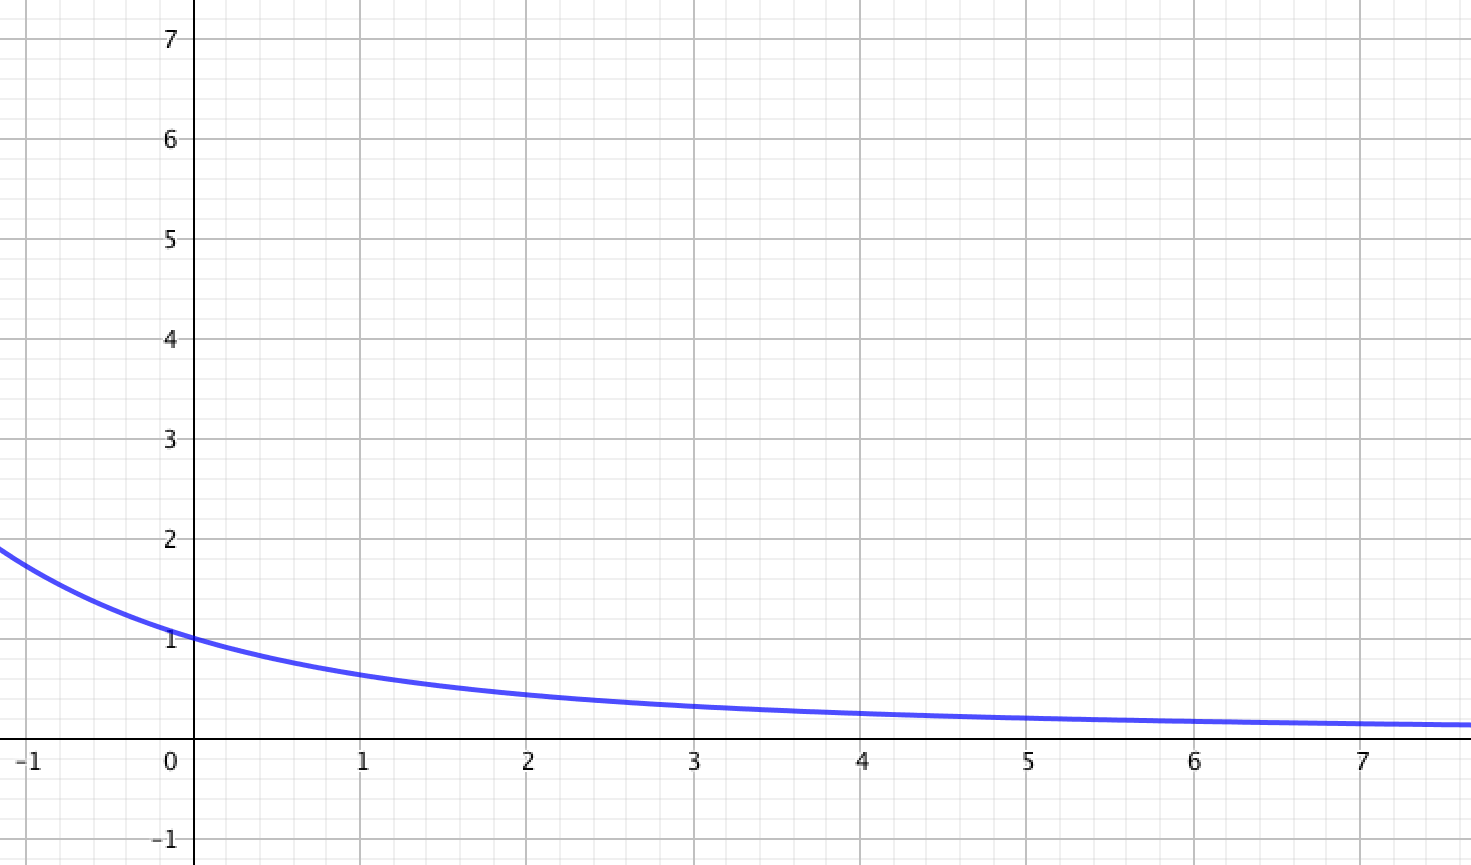
\includegraphics[width = 0.7 \textwidth]{Plot-Lemma3-15.png}
\caption{\label{fig: proofLemma3-15} Graph suggests our proof}
\end{figure}
A rigorous proof could be given using calculus.

\end{proof}


\begin{lemma}
For $t\geq1$, we have:
$$P(e^t)=\log(t)+M+\mathcal{O}(\frac{1}{t})$$
as $t$ goes to infinity.
\end{lemma}
\begin{proof}
Theorem \ref{Thm9Tenenbaum} gives
$$P(u)=M+\log(\log(u))+\mathcal{O}(\frac{1}{\log(u)})$$
Plugging in $u=e^t$ gives
$$P(e^t)=M+\log(\log(e^t))+\mathcal{O}(\frac{1}{\log(e^t)})$$
In other words
$$P(e^t)=M+\log(t)+\mathcal{O}(\frac{1}{t})$$
\end{proof}
\begin{definition}
$$f(x)=\sum_p\left(\frac{1}{2p^{2(x+1)}}+\frac{1}{3p^{3(x+1)}}+\frac{1}{4p^{4(x+1)}}\cdots \right)$$
\end{definition}

%$$=\sum_{p}\left(\log \frac{1}{1-p^{-1-x}}-p^{-1-x} \right)$$

\begin{lemma}
$f(x)$ converges uniformly for all $x\geq0$.
\end{lemma}
\begin{proof}
This is given from the argument in the proof of Lemma \ref{Sum leq zeta}.
\end{proof}

\begin{lemma}\label{log(zeta(1+x) integral}
We have the relation:
$$\log\left(\zeta(1+x)\right)=x \int_1^{\infty}e^{-xt}H(t)dt+\mathcal{O}(x)$$
as $x$ approaches $0$.
\end{lemma}
\begin{proof}
$$\log \left(\zeta(1+x)\right)= \log \left(\frac{1}{x}+ \mathcal{O}(1) \right)=\log \left(\frac{1}{x} \right)+\mathcal{O}(x)=\log \left( \frac{1}{1-e^{-x}} \right) + \mathcal{O}(x) $$
$$=\sum_{n=1}^{\infty}e^{-xn}n^{-1}+\mathcal{O}(x)=\int_{0}^{\infty}e^{-xt}dH(t)+\mathcal{O}(x)$$
$$=x \int_{1}^{\infty}e^{-xt}H(t)dt+\mathcal{O}(x)$$
The first step follows from Proposition \ref{gammaSondow}. The second step uses Lemma \ref{alex1}. The third step comes from Lemma \ref{alex3}. The fourth we get from the Taylor expansion of $\log$. The fifth expresses the infinite sum as a Riemann-Stieltjes integral, and the sixth comes from partial integration.
\end{proof}

\begin{lemma}
We have the relation:
$$G(x+1)=x\int
_0^{\infty}e^{-xt}P(e^t)dt$$
\end{lemma}
\begin{proof}
We can write
$$G(x+1)=\int_1^{\infty}u^{-x}dP(u)=x\int_1^{\infty}u^{-1-x}P(u)du=x\int
_0^{\infty}e^{-xt}P(e^t)dt$$
The first step expresses the prime zeta function as a Riemann-Stieltjes integral. The second is partial integration, and the third step comes from the substitution $u=e^t$.
\end{proof}

Recall that we are trying to prove Theorem \ref{fasterMTheorem}, and that what remains is to prove $M=\gamma-D$, or in other words $D=\gamma-M$. This is what we will prove now.

For $x>0$, we have (putting together all of the preceding lemmas)
\begin{equation}
\begin{split}
f(x) & =\sum_p\left(\frac{1}{2p^{2(x+1)}}+\frac{1}{3p^{3(x+1)}}+\frac{1}{4p^{4(x+1)}}\cdots \right) \\
& = \log(\zeta(x+1))-G(x+1) \\
& =x \int_1^{\infty} e^{-xt}H(t)dt+ \mathcal{O}(x)-x\int_0^{\infty}e^{-xt}P(e^t)dt \\
& =x \int_0^{\infty}e^{-xt}(H(t)-P(e^t))-x\int_0^{1}e^{-xt}P(e^t)dt+\mathcal{O}(x) \\
& =x \int_0^{\infty}e^{-xt}(H(t)-P(e^t))+\mathcal{O}(x) \\
& = x \int_1^{\infty}e^{-xt}\left(\gamma-M+\mathcal{O}\left(\frac{1}{t}\right)\right)dt + \mathcal{O}(x) \\
& = x \cdot (\gamma-M)\int_1^{\infty}e^{-xt}dt+x\int_1^{\infty}\mathcal{O}\left(\frac{1}{t}\right)\cdot e^{-xt}dt + \mathcal{O}(x) \\
& = (\gamma-M)e^{-x}+x\cdot C\cdot \int_1^{\infty}\frac{e^{-xt}}{t+1}dt+\mathcal{O}(x)
\end{split}
\end{equation}
Now, letting $x$ go to $0$ in the first and last expression, we get
$$D=\gamma-M$$
provided
$$x\cdot \int_1^{\infty}\frac{e^{-xt}}{t+1}dt \rightarrow 0$$
as $x$ goes to $0$.
We have not managed to prove this rigorously, but here is a graph of the entire expression as a function of $x$ which strongly indicates that this is true:
\begin{figure}[H]
\centering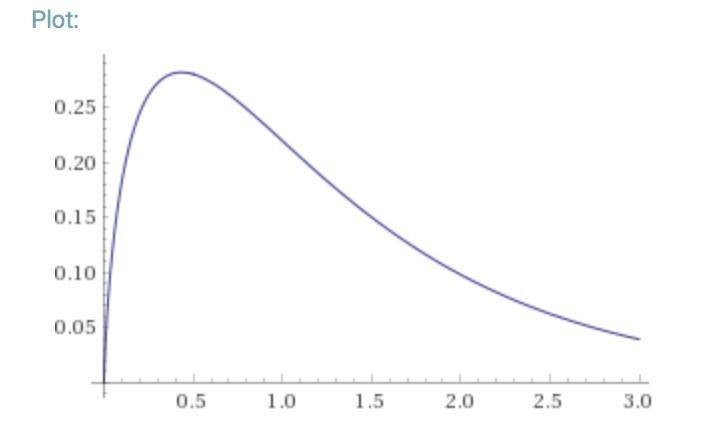
\includegraphics[width = 0.7 \textwidth]{PlotOfIntegral.jpg}
\caption{\label{fig: PlotOfIntegral} Plot of the integral expression}
\end{figure}
Wolfram Alpha also provides a proof that this limit is $0$, using the incomplete Gamma function, but we have not yet understood the details.

\subsection{Computational results with the faster algorithm}

In this subsection we use the theoretical results we found in the previous subsection to compute the classical Meissel-Mertens constant even better and faster.
\begin{example} \label{fasterMExample}
Here is our program which will do the computation:

\begin{figure}[H]
\centering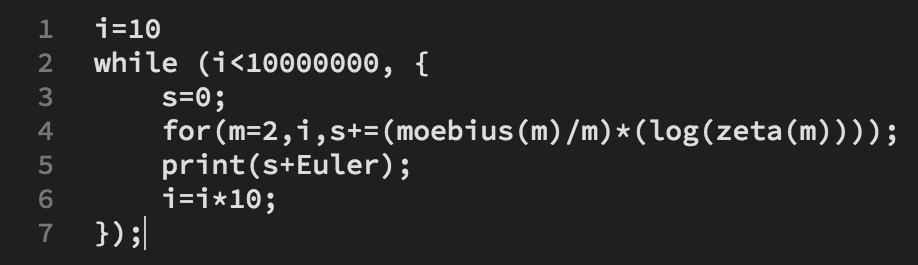
\includegraphics[width = 0.7 \textwidth]{classicalMFromFaster.png}
\caption{\label{fig: ClassicalMFromFaster} Efficient code for classical Meissel-Mertens constant}
\end{figure}
This program computes the following expression which we get from Theorem \ref{fasterMTheorem}:
$$\gamma + \sum_{m\geq 2} \frac{\mu(m)}{m}\cdot \log(\zeta(m))$$

Please note that this code is very efficient and will give many correct decimals. For this reason we will not be able to show the difference between some of them because of the lack of space on this paper.

\begin{table}[H]
\centering
\label{ClassicalMFromFaster}
\begin{tabular}{|l|l|}
\hline
$x$      & $M(F,x)$                                                                                                      \\ \hline
$10$     & $0.26154567382102619661695767828876711310231838667596386423105940601826634654599743$ \\ \hline
$10^2$ & $0.26149721284764278375542683860870284993031197675396849299802262190099476583338968$ \\ \hline
$10^3$ & $0.26149721284764278375542683860869585905156664826119920619206421392492451089736820$ \\ \hline
$10^4$ & $0.26149721284764278375542683860869585905156664826119920619206421392492451089736820$ \\ \hline
$10^5$ & $0.26149721284764278375542683860869585905156664826119920619206421392492451089736820$ \\ \hline
$10^6$ & $0.26149721284764278375542683860869585905156664826119920619206421392492451089736820$ \\ \hline
\end{tabular}
\caption{Classical Meissel-Mertens constants computed with the faster algorithm}
\end{table}
\end{example}
The last two constants in table 2 from example \ref{fasterMExample} have more than 400 identical decimals,  and these are identical to the Meissel-Mertens constant found in the OEIS-database\footnote{\url{http://oeis.org/A077761}}. Computation of all 6 values in the table above with 400 digits took 360ms in total with PARI/GP
\newpage

\section{Quadratic polynomials}
In this section we prove that $S(F)$ exists for any monic quadratic polynomial. We also show that there are three cases:

\subsection{Reducible polynomials}
For reducible polynomials, calculating the associated $a_p$ series can be done by factorising the polynomial.

\begin{example}\label{example 4.1}
If we for example take the polynomial $X^2-1$ we can find the $a_p$ series which is defined by the number of roots in $\mathbb{Z}/p$.
We start by factorising the polynomial:
$$X^2-1=(X-1)(X+1)$$
The factorisation makes counting roots easier. Let's evaluate the polynomial for some different $p$:
\begin{table}[H]
\centering
\begin{tabular}{c|c|c}
	\hline $p$ & roots & $a_p$ \\
	\hline $2$ & $X=1$ & $a_2=1$ \\
    \hline $3$ & $X=1$ , $X=2$ & $a_3 = 2$ \\
    \hline $5$ & $X=1$ , $X=4$ & $a_5 = 2$
\end{tabular}
\end{table}
We see that there will always be the two solutions $X=1$ and $X=p-1$, which implies that there is only one solution when $p=2$. If we want to calculate the Meissel-Mertens constant for this polynomial, we simply evaluate what the sum will look like:
\begin{equation} \label{eq2}
\begin{split}
& \sum_{p\leq n} \frac{a_p^2}{p} \\
& \frac{1}{2}+\frac{4}{3}+\frac{4}{5}+\frac{4}{7}\cdots
\end{split}
\end{equation}
By comparing to the expression for the Meissel Mertens constant, we see that the sum in (\ref{eq2}) can be written as
$$ \sum_{p\leq x}\frac{4}{p} - \frac{3}{2}$$
This gives us:
$$S(F)=\lim_{x \rightarrow \infty}\left(4\cdot \frac{\sum_{p\leq x}\frac{1}{p}-\frac{3}{2}}{\log(\log(x))}\right)$$
We can write this as:
$$S(F)=4\cdot \lim_{x \rightarrow \infty}\left(\frac{\sum_{p\leq x}\frac{1}{p}}{\log(\log(x))}-\frac{\frac{3}{2}}{\log(\log(x))}\right)$$
This we know to be $4\cdot 1 - 4\cdot 0 = 4$. In other words
$$S(F)=4$$
From this we get:
$$M(F,x)= \sum_{p\leq x}\frac{4}{p} - \frac{3}{2}-4\cdot \log(\log(x))$$
This implies
$$M(F)=4M-\frac{3}{2}\approx -0.45401114860942886$$
We compute in PARI with the naive algorithm:
\begin{figure}[H]
\centering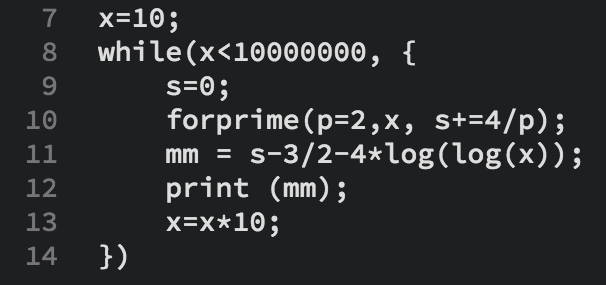
\includegraphics[width = 0.7 \textwidth]{Example4-1.png}
\caption{\label{fig: example4-1} Code for Meissel-Mertens constant for the reducible polynomial $X^2-1$}
\end{figure}
The code above evaluates the Meissel-Mertens constant for different limits so that we can see how the convergence  behaves. We get the following results:
\begin{table}[H]
\centering
\label{example4-1table}
\begin{tabular}{|l|l|}
\hline
$n$      & $M(F,n)$                                                  \\ \hline
$10$   & $-0.13136787622991843730809028666825162012272260870081$ \\ \hline
$10^2$ & $-0.39744969903612067739531737371686699081714631981958$ \\ \hline
$10^3$ & $-0.43825842696391179843992598455337237431063656558849$ \\ \hline
$10^4$ & $-0.44906743653714313015226382350002914809104934759758$ \\ \hline
$10^5$ & $-0.45279271453916810544566530551083579242914366970513$ \\ \hline
$10^6$ & $-0.45385525963335235307071642891508513073488546897224$ \\ \hline
\end{tabular}
\caption{Overview of M-values for the reducible polynomial $X^2-1$}
\end{table}

\end{example}

\begin{example}
Let's take the polynomial $X^2+6x-40$ and count roots the same way we did in the previous example.
We start by factorising the polynomial:
$$X^2+6x-40=(X+10)(X-4)$$
Now we evaluate the roots $\pmod{p}$:
\end{example}
\begin{table}[H]
\centering
\begin{tabular}{c|c|c}
	\hline $p$ & roots & $a_p$ \\
	\hline $2$ & $X=0$ & $a_2=1$ \\
    \hline $3$ & $X=1$ , $X=2$ & $a_3 = 2$ \\
    \hline $5$ & $X=0$ , $X=4$ & $a_5 = 2$ \\
    \hline $7$ & $X=4$ & $a_7 = 1$ \\
    \hline $11$ & $X=1$ , $X=4$ & $a_{11} = 2$
\end{tabular}
\end{table}
As in example \ref{example 4.1}, we see that the number of roots will be two, but with a couple of exceptions.
We can prove that $p=2$ and $p=7$ are the only cases where this happens.
\begin{proof}
The number of roots to this polynomial will be one when the following is true:
$$X+10 \equiv 0 \pmod{p} \quad \wedge \quad X-4 \equiv 0 \pmod{p}$$
\begin{equation}
\begin{split}
& X-4 \equiv X+10 \pmod{p} \\
\Leftrightarrow \quad & X-X \equiv 14 \pmod{p} \\
\Leftrightarrow \quad & 14 \equiv 0 \pmod{p} \\
\Leftrightarrow \quad & p | 14
\end{split}
\end{equation}
\end{proof}

Now let's see what this means for the sum:
$$\sum_{p \leq x}\frac{a_p^2}{p}$$
We know that $a_p=4$ except for $a_2=1$ and $a_7=1$. This gives us:
$$\sum_{p \leq x}\frac{a_p^2}{p}=\sum_{p \leq x}\frac{4}{p}-\frac{3}{2}-\frac{3}{7}$$
Hence,
$$S(F)=\lim_{x \rightarrow \infty}\left(4\cdot \frac{\sum_{p\leq x}\frac{1}{p}-\frac{3}{2}-\frac{3}{7}}{\log(\log(x))}\right)$$
As in example \ref{example 4.1} we now write
$$S(F)=4\cdot \lim_{x \rightarrow \infty}\left(\frac{\sum_{p\leq x}\frac{1}{p}}{\log(\log(x))}-\frac{\frac{3}{2}}{\log(\log(x))}-\frac{\frac{3}{7}}{\log(\log(x))}\right)$$
$$S(F)=4\cdot \lim_{x \rightarrow \infty}\left(\frac{\sum_{p\leq x}\frac{1}{p}}{\log(\log(x))}\right)-\lim_{x \rightarrow \infty}\left(\frac{\frac{3}{2}}{\log(\log(x))}\right)-\lim_{x \rightarrow \infty}\left(\frac{\frac{3}{7}}{\log(\log(x))}\right)$$
$$S(F)=4-0-0$$
$$S(F)=4$$

\begin{theorem}
For any reducible monic quadratic polynomial $F$ with discriminant $0$, we have
$$S(F)=1$$
\end{theorem}
\begin{proof}
We can write $F$ as
$$(X+a)(X+b)$$
The discriminant is zero when $a=b$.
When $a=b$, we see that the number of roots $\mathbb{Z}/p$ is one for all primes. When $a_p=1 \quad \forall \quad p$, the expression for $S(F)$ is identical to the one we had for a monic linear polynomial, and we get $S(F)=1$.
\end{proof}
\begin{theorem}\label{preben1}
For any reducible quadratic monic polynomial $F$ with non-zero discriminant, we have
$$S(F)=4$$
\end{theorem}
\begin{proof}
The first step in our proof will be to show that $a_p(F)$ always is $2$ except for a few special cases where it is $1$.
First, we observe that any reducible monic quadratic polynomial, by definition, can be factorized, and thus we can write:
$$F(X)=(X+a)(X+b)$$
where $a$ and $b$ are integers.
Now
\begin{equation}\label{F(X) is 0}
F(X) \equiv 0 \pmod{p}
\end{equation}
gives
$$(X+a)\equiv 0 \pmod{p} \quad \vee \quad (X+b) \equiv 0 \pmod{p}$$
It is trivial that both of these equations will have one solution, and one solution only. Therefore there will always be two solutions for (\ref{F(X) is 0}) except when $a\equiv b \pmod{p} $.
We now need to show that this only happens for a finite number of values of $p$.
\begin{equation}
\begin{split}
& a \equiv b \pmod{p} \\
\Leftrightarrow \quad & a-b \equiv 0 \pmod{p} \\
\Leftrightarrow \quad & p \vert (a-b)
\end{split}
\end{equation}
This means that $p$ is a factor in $(a-b)$. Now $(a-b)$ is an integer, and any integer has by definition only a finite number of prime factors. Hence, $p \vert (a-b)$ only for a finite number of primes $p$.
We have $a_p=2$ for all primes $p$ except the ones such that $p \vert (a-b)$. From this we can write:
$$\sum_{p}\frac{a_p^2}{p}=\sum_{p}\frac{4}{p}-\sum_{p \vert (a-b)}\frac{3}{p}$$
We insert this into $S(F)$, and get
$$S(F)=\lim_{n \rightarrow \infty}\left(\frac{\sum_{p}\frac{4}{p}-\sum_{p \vert (a-b)}\frac{3}{p}}{\log(\log(n))} \right)$$
Once again we can rewrite
$$4\cdot \lim_{n \rightarrow \infty}\left(\frac{\sum_{p\leq n}\frac{1}{p}}{\log(\log(n))}\right)-\lim_{n \rightarrow \infty}\left(\frac{\sum_{p \vert (a-b)}\frac{3}{p}}{\log(\log(n))}\right)$$
This is
$$4-0$$
so we arrive at
$$S(F)=4$$
\end{proof}

\subsection{Irreducible polynomials}
In this subsection we show how we can use the Kronecker symbols to find the sequence $a_p$ for irreducible quadratic polynomials.
\begin{lemma} \label{Lemma1}
Set $F(X)=X^2-k$ and F irreducible, and let $p$ denote an odd prime:
\newline
The number of solutions to $$F(X)\equiv 0 \pmod{p}$$
is exactly $$1+\left(\frac{k}{p}\right)$$
where $(\frac{k}{p})$ is the Legendre symbol.
\end{lemma}
\begin{proof}
$$F(x)\equiv 0 \pmod{p} \Leftrightarrow  X^2\equiv k \pmod{p}$$
We can separate this into three different cases:
$$= \begin{cases}
1  & \text{if } a \equiv 0\pmod{p} \\
2 & \text{if } a \not\equiv 0\pmod{p} \text{ and for some integer } x\colon\;a\equiv x^2\pmod{p},\\
0 & \text{if } a \not\equiv 0\pmod{p} \text{ and there is no such } x.
\end{cases}$$
We see that, assuming p is odd, this is exactly the same as $1+(\frac{k}{p})$
\end{proof}
\begin{proposition} \label{alex5}
Let $p$ denote any odd prime and set $F=X^2+bX+c$ and F irreducible.
The number of roots to the polynomial F in $\mathbb{Z}/p$ is exactly: $$1+\left(\frac{b^2-4c}{p}\right)$$
\end{proposition}
\begin{proof}
We calculate in $\mathbb{Z}/p$:
\begin{equation}
\begin{split}
& X^2+bX+c=0 \\
 \Leftrightarrow 4&X^2+4bX+4c=0 \\
 \Leftrightarrow (2&X+b)^2-b^2+4c = 0 \\
 \Leftrightarrow (2&X+b)^2-(b^2-4c) = 0 \\
\end{split}
\end{equation}
We substitute
$$u=2X+b, k=b^2-4c$$
This gives us the equivalence
$$X^2+bX+c=0 \Leftrightarrow u^2-k=0$$
As shown in \ref{Lemma1} the number of solutions $u^2-k=0$ is $1+(\frac{k}{p})=1+(\frac{b^2-4c}{p})$.
Because $u=2X+b$, we see that every $u$ gives only one $X$ and vice versa (this uses the fact that p is odd).
\end{proof}

\begin{theorem} \label{kronecker}
Let $F$ be any irreducible quadratic polynomial of the form $X^2+bX+c$, let $d$ denote the discriminant $b^2-4c$ and let $(\frac{\cdot}{n})$ denote the Kronecker symbol.
The number of solutions to $F(X)\equiv 0 \pmod {p}$ is:
$$1+\left(\frac{d}{p}\right)$$
\end{theorem}
\begin{proof}
We separate the proof into two cases: The first case is when $p$ denotes any odd prime and the second case is when $p=2$.
For $p$ an odd prime, Proposition \ref{alex5} already proved that the number of solutions $F(x)\equiv 0 \pmod {p}$ is:
$$1+\left(\frac{d}{p}\right)$$
For the case $p=2$, though, we prove by exhaustion. When calculating $\pmod{2}$ we observe that there only really exist four different cases for $F=X^2+bX+c$:

$$F_1(X)=X^2 \quad , \quad d=0$$
$$F_2(X)=X^2+X \quad , \quad d=1$$
$$F_3(X)=X^2+1\quad , \quad d=-4$$
$$F_4(X)=X^2+X+1\quad , \quad d=-3$$

For our proof to be complete we only need to show that the formula holds for these polynomials. We can list the solutions to each of the four congruences as follows:
$$F_1\equiv0\pmod{2} \text{ when } X=0$$
$$F_2\equiv0\pmod{2} \text{ when } X=0 \text{ and } X=1$$
$$F_3\equiv0\pmod{2} \text{ when } X=1$$
$$F_4\equiv0\pmod{2} \text{ for no value of }X$$
For $F_1$ we have one solution, for $F_2$ we have two, for $F_3$ we have one and for $F_4$ we have zero solutions. At the same time, we can compute:
$$1+\left(\frac{d}{p}\right)=1+\left(\frac{0}{2}\right)=1+0=1$$
$$1+\left(\frac{d}{p}\right)=1+\left(\frac{1}{2}\right)=1+1=2$$
$$1+\left(\frac{d}{p}\right)=1+\left(\frac{-4}{2}\right)=1+0=1$$
$$1+\left(\frac{d}{p}\right)=1+\left(\frac{-3}{2}\right)=1+(-1)=0$$
This equals the number of solutions, and thereby concludes our proof.
\end{proof}


\subsection{Convergence proofs}
We fix an integer $k$ and let $K(p)$ denote the Kronecker symbol $\left(\frac{k}{p}\right)$.
\begin{lemma}\label{Original S(F)}
$$\lim_{n \rightarrow \infty} \frac{\sum_{p \leq n}\frac{1}{p}}{\log(\log(n))}=1$$
\end{lemma}
\begin{proof}
This was proved in Lemma \ref{S is 1}.
\end{proof}


\begin{lemma}
K is a Dirichlet character.
\end{lemma}
\begin{proof}
This is well known. See the Wikipedia article on Kronecker symbols. \footnote{\url{https://en.wikipedia.org/wiki/Kronecker_symbol}}
\end{proof}

\begin{lemma}\label{Limit from Kedlaya}
The limit
$$\lim_{n \rightarrow \infty}\sum_{p\leq n}\frac{K(p)}{p}$$
exists.
\end{lemma}
\begin{proof}
It is known that sum
$$\sum_{n=1}^{\infty}\frac{\chi(n)}{n^x}$$
converges for any $x \geq 0$. See for example lecture 5 of Kedlaya's lecture notes. \footnote{MIT lecture notes on Analytic Number Theory, K. S. Kedlaya}
Now the lemma follows from an argument with Euler products identical to the argument in Lemma \ref{logzeta-G}.
\end{proof}

\begin{lemma}\label{2limK(p)}
We have
$$\lim_{n \rightarrow \infty} \frac{\sum_{p\leq n}\frac{K(p)}{p}}{\log(\log(n))}=0$$
\end{lemma}
\begin{proof}
From \ref{Limit from Kedlaya} we can conclude that the sum in our numerator will be finite. Because $\log(\log(n))$ approaches infinity as n approaches infinity the expression has to be zero.
\end{proof}
\begin{lemma}\label{K(p) squared}
We have
$$\lim_{n \rightarrow \infty}\frac{\sum_{p \leq n}\frac{K(p)^2}{p}}{\log(\log(n))} =1$$
\end{lemma}
\begin{proof}
From the definition of the Kronecker symbol, \ref{defKronecker} we know that our denominator can only be zero or one, and that it is zero when $p$ is a factor in $k$. We have
$$\lim_{n \rightarrow \infty}\frac{\sum_{p \leq n}\frac{K(p)^2}{p}}{\log(\log(n))} =1$$
Let's look at the numerator:
$$\sum_{p \leq n}\frac{K(p)^2}{p}$$
When $p\vert k$, the numerator is zero. We get:
$$\sum_{p \leq n}\frac{K(p)^2}{p}+\sum_{p\vert k}\frac{1}{p}=\sum_{p\leq n}\frac{1}{p}$$
$$\sum_{p \leq n}\frac{K(p)^2}{p}=\sum_{p\leq n}\frac{1}{p}-\sum_{p\vert k}\frac{1}{p}$$
Inserting this into the original expression we get:
$$\lim_{n \rightarrow \infty}\frac{\sum_{p\leq n}\frac{1}{p}-\sum_{p\vert k}\frac{1}{p}}{\log(\log(n))}$$
which is equal to
$$\lim_{n \rightarrow \infty}\left(\frac{\sum_{p\leq n}\frac{1}{p}}{\log(\log(n))}-\frac{\sum_{p\vert k}\frac{1}{p}}{\log(\log(n))}\right)$$
Because $\sum_{p\vert k}\frac{1}{p}$ is a finite sum, we have
$$\lim_{n \rightarrow \infty}\left(\frac{\sum_{p\vert k}\frac{1}{p}}{\log(\log(n))}\right)=0$$
Together with Lemma \ref{Original S(F)} this concludes our proof.
\end{proof}
\begin{theorem}\label{S is 2}
For any monic quadratic irreducible polynomial $F$ we have $S(F)=2$.
\end{theorem}
\begin{proof}
In subsection 2.3 we showed that $a_p = 1+(\frac{d}{p})$ where $d$ is the discriminant of $F$. This gives us $a_p^2=1+2(\frac{k}{p})+(\frac{k}{p})^2$ Now we start to calculate $S(F)$:
\begin{equation}
\begin{split}
& S(F)=\lim_{n \rightarrow \infty} \frac{\sum _{p\leq n}\frac{1+2(\frac{d}{p})+(\frac{d}{p})^2}{p} }{\log(\log(n))} \\
& = \lim_{n \rightarrow \infty} \frac{\sum_{p \leq n}\frac{1}{p}}{\log(\log(n))} + 2\cdot \lim_{n \rightarrow \infty} \frac{\sum_{p\leq n}\frac{(\frac{d}{p})}{p}}{\log(\log(n))} + \lim_{n \rightarrow \infty}\frac{\sum_{p \leq n}\frac{(\frac{d}{p})^2}{p}}{\log(\log(n))}
\end{split}
\end{equation}
From Lemma \ref{Original S(F)}, Lemma \ref{2limK(p)} and Lemma \ref{K(p) squared} we know that this is $1+0+1=2$.
\end{proof}

\begin{theorem}
The limit
$$M(F) = \lim_{n\rightarrow\infty}\left(\sum_{p\leq n}\frac{a_p^2}{p} - S(F)\cdot \log(\log(n)) \right)$$
exists for all monic quadratic polynomials.
\end{theorem}
\begin{proof}
Let $F$ be any irreducible monic quadratic polynomial.
$$M(F) = \lim_{n\rightarrow\infty}\left(\sum_{p\leq n}\frac{a_p^2}{p} - S(F)\cdot \log(\log(n)) \right)$$
From Theorem \ref{S is 2}. this can be written as,
$$\lim_{n\rightarrow\infty}\left(\sum_{p\leq n}\frac{1}{p}+2\cdot \sum_{p \leq n}\frac{K(p)}{p}+\sum_{p \leq n}\frac{1}{p} - \sum_{p\vert k}\frac{1}{p} - 2\cdot \log(\log(n)) \right)$$
By simplifying, we get,
$$\lim_{n \rightarrow \infty}\left(2\cdot \sum_{p \leq n}\frac{1}{p}-2\log(\log(n))+C\right)$$
where we have set
$$C=2\cdot \sum_{p \leq n}\frac{K(p)}{p}- \sum_{p\vert k}\frac{1}{p}$$
From Lemma \ref{Limit from Kedlaya} and Lemma \ref{K(p) squared} we know that $C$ is a constant. Hence, we can write,
$$2\cdot \lim_{n \rightarrow \infty}\left(\sum_{p \leq n}\frac{1}{p}-\log(\log(n))\right)+C$$
This limit is the original Meissel-Mertens constant, and therefore our theorem holds for irreducible polynomials.

For $F$ a reducible monic quadratic polynomial, the proof is similar using the results of section $4.1$.
\end{proof}

\subsection{Computational results with the naive algorithm}
In this subsection we use our theoretical results to compute constants for different quadratic, irreducible and monic polynomials.


\begin{example}
This is a table with some numerical results for $S(F)$. Here $d$ denotes the discriminant $b^2-4c$.
\begin{table}[H]
\centering
\begin{tabular}{c|c|c|c|c|c|c|c}
	\hline
	 & $n$ & $X^2-X+1$& $X^2+1$ & $X^2-X-1$ & $X^2-X+4$ & $X^2+2$\\
	\hline\hline
	d & & -3 & -4 & 5 & -15 & -8 \\
	\hline
&	$10^6$ & 1.552706 & 1.735751 &1.921039 & 2.214302 & 2.002109\\
	\hline
&	$2\cdot 10^6$ & 1.563067 & 1.741746 &1.922784 & 2.208929 & 2.001670\\
	\hline
&	$3\cdot 10^6$ & 1.568413 & 1.744931 &1.923801 & 2.206173 & 2.001471\\
	\hline
&	$4\cdot 10^6$ & 1.572251 & 1.744931 &1.924478 & 2.204360 & 2.001492\\
	\hline
&	$5\cdot 10^6$ & 1.575098 & 1.748827 &1.924983 & 2.202903 & 2.001607\\
	\hline
&	$6\cdot 10^6$ &1.577385& 1.750188 &1.925366 & 2.201859 & 2.001555\\
	\hline
&	$7\cdot 10^6$ & 1.579197 & 1.751275 &1.925655 & 2.200965 & 2.001522\\
	\hline
&	$8\cdot 10^6$ & 1.580759 & 1.752155 &1.925874 & 2.200273 & 2.001529\\
	\hline
&	$9\cdot 10^6$ & 1.582172 & 1.752986 &1.926072 & 2.199618 & 2.001533\\
	\hline
&	$10 \cdot 10^6$& 1.583393 & 1.753641 & 1.926233 & 2.199000 & 2.001463\\
	\hline
\end{tabular}
\caption{S(F)}
\label{S(F) numerically for some polynomials deg2}
\end{table}

These are just a sample of many polynomials we tested (see the link in the footnote below for more values \footnote{\url{https://goo.gl/SPHWoH}}).
We also see how obvious it is that all constants go to $2$ as n goes to $\infty$.
\end{example}

\begin{example}
Here is a quick overview of how our code in PARI/GP will look like when we compute the Meissel-Mertens constant for a quadratic polynomial:

\begin{figure}[H]
\centering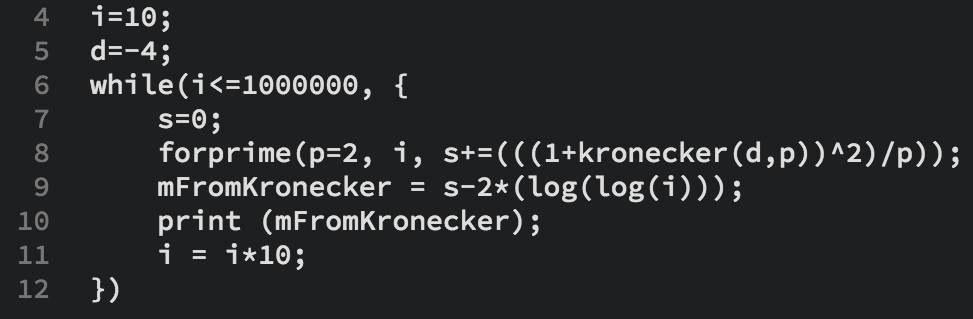
\includegraphics[width = 0.7 \textwidth]{mFromKronecker-d-4.png}
\caption{\label{fig: Kroneckertest} Code for Meissel-Mertens constant from Kronecker symbols for polynomial $X^2+1$}
\end{figure}
We use one of the simplest quadratic polynomials $X^2+1$ with the discriminant $d = -4$ for our first example. The expression represented in the program above is:
$$\sum_{p\leq x} \frac{a_p^2}{p}-2\cdot \log\log(x))$$
where
$$a_p = 1+\left(\frac{d}{p}\right)$$
and $d$ is the polynomial's discriminant. We will show how $a_p$ will look like just to visualize the series:
$$a_2 = 1, \quad a_3 = 1, \quad a_5 = 1, \quad a_7 = 2, \quad a_{11} = 2, \quad a_{13} = 0, \quad a_{17} = 2, \quad a_{19} = 0, \quad a_{23} = 0, \quad a_{29} = 0$$
\newline
We also vary the limit $n$ to see how fast the constant converges.

The program above gives us the result:
\begin{table}[H]
\centering
\label{example4-3table}
\begin{tabular}{|l|l|}
\hline
$n$      & $M(F,n)$                                                     \\ \hline
$10$   & $-0.3680648904959115996064261$ \\ \hline
$10^2$ & $-0.5857517852960758881135608$ \\ \hline
$10^3$ & $-0.6355227896330265581011639$ \\ \hline
$10^4$ & $-0.6418758426123608795376946$ \\ \hline
$10^5$ & $-0.6456835969379260796530403$ \\ \hline
$10^6$ & $-0.6468859103902465117460938$ \\ \hline
\end{tabular}
\caption{Overview over M-values for polynomial $X^2+1$}
\end{table}
\end{example}

Here is a sample of some of the constants we computed for different polynomials. Many more examples can be found in [\ref{refSpreadsheet}].
\begin{table}[H]
\centering
\begin{tabular}{c|c|c|c|c|c|c|c}
	\hline
	 & $n$ & $X^2-X+1$& $X^2+1$ & $X^2-X-1$ & $X^2-X+4$ & $X^2+2$\\
	\hline\hline
	d & & -3 & -4 & 5 & -15 & -8 \\
	\hline
&	$10^6$ & -1.092947 & -0.645683 &-1.69191 & 0.523642 & 0.005154\\
	\hline
&	$2\cdot10^6$ & -1.093177 & -0.646133 &-1.69241 & 0.522728 & 0.004179\\
	\hline
&	$3\cdot10^6$ & -1.093905 & -0.646133 &-1.69273 & 0.522570&  0.003730\\
	\hline
&	$4\cdot10^6$ & -1.093824 & -0.646485 &-1.69252 & 0.522585 & 0.003815\\
	\hline
&	$5\cdot10^6$ & -1.093830 & -0.646597 &-1.69244 & 0.522339 & 0.004137\\
	\hline
&	$6\cdot10^6$ &-1.093774  & -0.646541 &-1.692675 &0.522436 & 0.004024 \\
	\hline
&	$7\cdot10^6$ & -1.093932 & -0.646592 &-1.692717 &0.522438  &0.003957 \\
	\hline
&	$8\cdot10^6$ & -1.094010 & -0.646751 &-1.692750 &0.522615  &0.003991 \\
	\hline
&	$9\cdot10^6$ & -1.093928 & -0.646714 &-1.692754 &0.522627  &0.004014 \\
	\hline
&	$10\cdot10^6$ & -1.093922 & -0.64688 &-1.692777 &0.522533  &0.003842 \\
	\hline
\end{tabular}
\caption{M(F,n) for some quadratic, irreducible and monic polynomials}
\label{M(F) numerically for some polynomials deg2}
\end{table}
\newpage
\section{Work in progress}
\subsection{Cubic polynomials}

We have been looking into cubic polynomials to see if we can apply the same techniques as the ones we found in section 3 and 4, as well as some theory from Dedekind zeta-functions.
We have many numerical experiments for cubic polynomials but we have not proved any theoretical results yet.


\subsection{Theory for faster computation of quadratic polynomials}
We are currently trying to find an expression for $M(F)$ for quadratic polynomials similar to the one we found in section 3.4 for linear polynomials, by for example changing the Riemann zeta-function with an L-function for a given number field defined by the polynomial in question. Some of the test runs in computing this has been almost satisfying but we are still looking for the solution.


\newpage



\begin{thebibliography}{9}
\bibitem{Murty}\label{refMurty}
M.Ram Murty. \textit{Selberg's conjectures and Artin L-functions, American mathematical society July 1994, volume 31, number 1, \url{https://arxiv.org/abs/math/9407219}}
\bibitem{Analytic L-functions}
David W. Farmer, Ameya Pitale, Nathan C. Ryan,
and Ralf Schmidt \textit{Analytic L-functions: definitions,
theorems, and connections, \url{https://arxiv.org/abs/1711.10375}}
\bibitem{Selberg}
M.Scott Osborne, Garth Warner. \textit{Selberg trace formula III: Inner product formulae, American mathematical society July 1983 volume 44 number 283, }
\bibitem{Tenenbaum} \label{refTenenbaum}
Gerald Tenenbaum. \textit{Introduction to Analytic and Probabilistic Number Theory (Graduate Studies in Mathematics) 3rd Edition
}
\bibitem{Hardy}
G.H. Hardy, E.M. Wright. \textit{An introduction to the theory of numbers}
\bibitem{Languasco}
Alessandro Languasco, Alessandro Zaccagnini. \textit{computing the Mertens and Meissel-Mertens constants for sums over arithmetic progressions}
\bibitem{Wikipedia:Dirichlet} Wikipedia article on Dirichlet Characters \url{https://en.wikipedia.org/wiki/Dirichlet_character}
\bibitem{Sondow}\label{sondowRef}
Jonathan Sondow. \textit{An antisymmetric formula for Euler's constant}, Mathematics magazine, Vol. 71 No. 3 (June 1998)
\bibitem{K.S. Kedlaya}
Lecture notes on analytic number theory from MIT Open CourseWare (2007), \url{https://dspace.mit.edu/bitstream/handle/1721.1/101679/18-785-spring-2007/contents/lecture-notes/index.htm}
\bibitem{Big O Notation}
Wikipedia article on Big O Notation \url{https://en.wikipedia.org/wiki/Big_O_notation}
\bibitem{Primezeta} Mathworld.wolfram article on the Prime Riemann zeta function: \url{http://mathworld.wolfram.com/PrimeZetaFunction.html}
\bibitem{Spreadsheet} \label{refSpreadsheet} Spreadsheet with our computational results: \url{https://docs.google.com/spreadsheets/d/19s5vXErSTEA1XtY1qd2K4TUnhOMISlJyqDfwHnJSwJk/edit?usp=sharing}
\bibitem{The Möbius function}
Wikipedia article on the Möbius function \url{https://en.wikipedia.org/wiki/Möbius_function}
\bibitem{KroneckerSymbols} Wikipedia article on the Kronecker symbol: \url{https://en.wikipedia.org/wiki/Kronecker_symbol#Connection_to_Dirichlet_characters}
\bibitem{Flajolet}\label{refFlajolet} Philippe Flajolet, Ilan Vardi \textit{Zeta function expansions of classical constants} February 24, 1996
\bibitem{Mazur} Barry Mazur, William A. Stein,  \textit{Prime numbers and the Riemann hypothesis}
\bibitem{Proof of the Eueler product formula for the Riemann zeta function} Wikipedia article which presents a proof for the Euler product formula for the Riemann zeta function:
\url{https://en.wikipedia.org/wiki/Proof_of_the_Euler_product_formula_for_the_Riemann_zeta_function#Another_proof}
\end{thebibliography}
\end{document}
